% !TeX program = lualatex

\documentclass[12pt]{report}
\usepackage[Glenn]{fncychap}
\usepackage[T1]{fontenc}
\usepackage[francais]{babel}
\usepackage{fontspec}
\usepackage{wrapfig}
\usepackage{graphicx}
\usepackage{subcaption}
\usepackage{caption}
\usepackage{soul}
\usepackage[colorlinks=true, linkcolor=black, urlcolor=black, citecolor=black]{hyperref}
% \usepackage[hyphens, spaces, obeyspaces]{url}
\usepackage[a4paper, width=175mm, top=25mm, bottom=25mm]{geometry}
\usepackage{parskip}
\usepackage{enumitem}
\usepackage{titlesec}
\usepackage{listings}
\usepackage{float}
\usepackage[final]{pdfpages}
\usepackage{xcolor}
\usepackage{tocbibind}
\usepackage{tocloft}
\usepackage{xpatch}
\usepackage{amsmath}
\usepackage{amsthm}
\usepackage{amsfonts}
\usepackage{graphics}
\usepackage{color}
% \usepackage[grey,utopia]{quotchap}
\usepackage{moreverb}
\usepackage{xcolor}
\usepackage{framed}
%\usepackage{arabluatex}
%\usepackage[algo2e, french, onelanguage, ruled]{algorithm2e}
\setlist[itemize]{label=\textbullet}
\usepackage{fancyhdr}
\pagestyle{fancy}   
\fancyhead{}
\fancyhead[C]{\leftmark}
\renewcommand{\headrulewidth}{0.4pt}
\renewcommand{\footrulewidth}{0.4pt}
\usepackage{xcolor}
\definecolor{light-gray}{gray}{0.90}
\usepackage{multirow}
\usepackage{soul}
\usepackage[utf8x]{inputenc}
\setcounter{secnumdepth}{3} 
\usepackage{dirtytalk}
\usepackage{csquotes}
\usepackage{mathtools}
\usepackage{amsmath}
\begin{document}
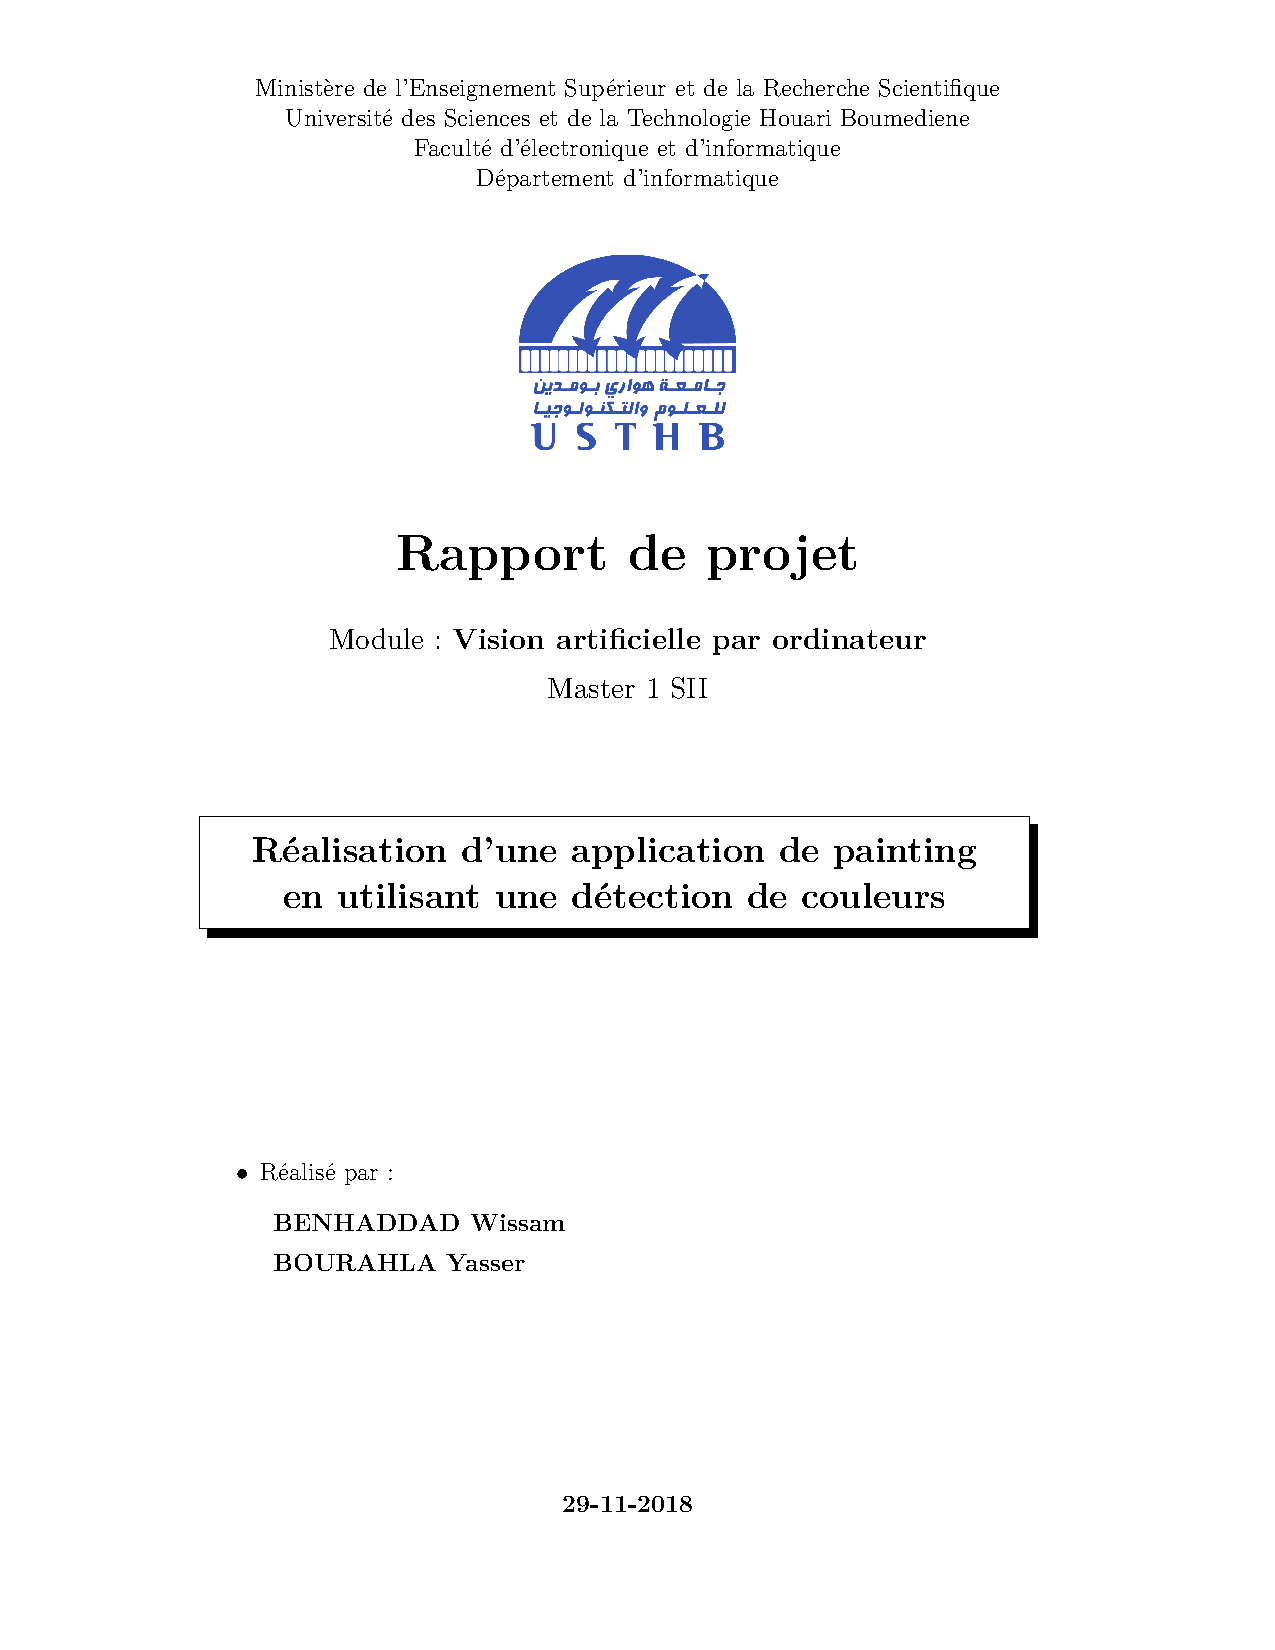
\includepdf[pages=1]{Page_garde.pdf} 
\tableofcontents
\listoffigures
\listoftables


\pagenumbering{arabic}
\newpage

\setlist[itemize]{label=\textbullet}
\chapter{Introduction}
	\section{Problématique et objectifs }
	\paragraph{}
	La vision par ordinateur est un domaine très vaste et dont les domaines d'application sont
	divers et variés, comme introduction à ce nouveau domaine, nous avons pour but dans ce projet
	de réaliser une petite application de painting en utilisant la détection de couleurs sur une 
	séquence d'images prises depuis une caméra.
	\par 
	Le but principale derrière ce projet est la familiarisation avec les outils théorique vus en cours,
	ainsi que l'utilisation de ces derniers en pratique. La difficulté réside aussi dans l'élaboration
	d'un système robuste (dans la limite du possible) au bruit et aux conditions d'utilisation.
	\par 
	Le rapport est divisé en 3(trois) chapitres, le premier se concentrera sur des définitions formelles
	des concepts et technique que nous utiliserons dans notre système. Le chapitre suivant présentera
	plus de détails sur notre système, ses composants, son fonctionnement interne, ainsi qu'une brève
	explication de notre filtre anti-bruits. Puis nous enchaînerons sur une présentation de notre
	application. Enfin nous conclurons par une analyse des méthodes utilisées et les différentes 
	approches et perspectives futures.
	
	\section{Définitions}
	\paragraph{}
	Comme mentionné plus haut, nous allons commencer par quelques définitions que nous avons jugées 
	importantes pour la suite de ce rapport.
	
		\subsection{Une image sous différents angles}
		\paragraph{}
		Puisque nous allons travailler sur une séquence d'image(aussi appelée video), nous devons
		d'abord définir ce qu'est une image d'un point de vu artificielle.
		\par
		Il existe plusieurs représentations d'une image sur ordinateur, la plus connue reste la 
		représentation matricielle, où une image 2D est codifié dans une matrice $M_{n,m}$ de 
		dimensions $n\times m$ ($lignes \times colones$), chaque entrée $a_{i,j}$dans cette matrice 
		représente la plus petite unité d'une image appelé \textbf{pixel}, un pixel peut prendre
		plusieurs valeurs selon l'espace de représentation qu'on associe à l'image, nous avons
		travaillé essentiellement avec trois représentations : 
		\begin{itemize}
			\item représentation \textbf{RVB} : chaque pixel est composé de 3 valeurs pour chaque
			couleur primaires appartenant à l'intervalle $\left[0,255\right]$, ainsi ce pixel sera
			un mélange des composantes Rouge,Vert,Bleu
			
			\item représentation par niveau de gris : analogue à la représentation précédente, 
			le pixel prend la valeur moyenne des trois composantes $\frac{r+v+b}{3}$, le résultat 
			est une valeur de niveau de gris allant de $0$(noir) à $255$(blanc).
			
			\item représentation dans l'espace \textbf{HSV} : ici un pixel sera aussi composé
			de trois valeurs, mais leur signification sera différente, le \textbf{H}(Hue) ou
			la teinte représente quelle couleur le pixel prendra, \textbf{S}(Saturation) l'intensité
			de la couleur choisi, une grande valeur signifie une couleur vive, et une petite valeur
			signifie une couleur pâle(grisâtre), \textbf{V}(Value) la luminosité est la quantité de 
			lumière présente dans l'image, plus elle est petite plus l'image est sombre(tend vers le noir),
			inversement plus elle est grande plus l'image est vibrante(lumineuse).
		\end{itemize} 
		\subsection{Notion de vidéo}
		\paragraph{}
		Une vidéo est une collections d'images successives ou \textbf{trames} qui défilent à
		une certaine cadence, donnant l'illusion d'un mouvement continu à travers le temps.
		
		\subsection{Opération sur les images}
		\paragraph{}
		Une image sous la forme matricielle peut être soumise à plusieurs type d'opération arithmétiques(addition,
		soustraction, multiplication ...) ou ensemblistes(intersection, union ...). Une opération bien
		connue dans le domaine est la convolution, en bref c'est une opération de transformation de l'image
		à par le biais d'un élément structurant(image plus petite, carré, cercle ...), l'idée est qu'en 
		superposant un élément structurant sur un pixel de l'image, le pixel à la même position peut être 
		transformé comme combinaison linéaire(pas forcement linéaire) des pixel voisins du pixel orignal et
		celui de l'élément structurant, en appliquant ce principe nous définissons ces quatre type de filtres :
		
			\subsubsection{Filtre moyen}
			\paragraph{}
			Le filtre moyen transforme la valeur du pixel central en une moyenne de ces voisins, cette opération 
			à tendance tendance à contaminer les valeurs voisines avec cette valeur aberrante et flouter l'image,
			
			\subsubsection{Filtre médiane}
			\paragraph{}
			Le filtre médian est un filtre numérique non linéaire, visant à remplacer les pixels centraux par 
			la valeur médiane de ses voisins, il est souvent utilisé pour la réduction de bruit tout en conservant
			le contraste de l'image
			
			\subsubsection{Dilatation}
			\paragraph{}
			
			La dilatation est un filtre morphologique non-linéaire visant à dilater les objets d'une image.
			Soit $X$ une image, à savoir un ensemble de pixels. Pour un élément structurant $B$, la dilatation
			de $X$ par $B$ est l'ensemble obtenu en remplaçant chaque pixel $p$ de $X$ par sa fenêtre $Bp$ :
			$DilB(X) =  {Bp | p  X}$.
			L'effet de la dilatation est d'abord d'élargir la figure, la hauteur et largeur de la figure dilatée seront les sommes respectivement des hauteurs et largeurs de la figure originelle et de l'élément structurant. Si l'élément structurant est décentré, la dilatation décalera la figure dans le même sens. Enfin les coins convexes de la figure seront déformés en fonction de l'élément structurant (par exemple si celui-ci est un disque, les coins convexes seront arrondis).
			
			\subsubsection{Érosion}
			\paragraph{}
			L'érosion est aussi un filtre morphologique non-linéaire.
			Soit $X$ la même image, et $B$ un élément structurant. L'érosion de $X$ par $B$ est l'ensemble des pixels p tels que la fenêtre $Bp$ est incluse dans X :
			$ErosB(X) = {p | Bp  X}$.
			L'effet de l'érosion est d'abord de rétrécir la figure, la hauteur et largeur de la figure érodée seront les différences respectivement des hauteurs et largeurs de la figure originelle et de l'élément structurant (en particulier si l'élément structurant est plus large ou plus haut que la figure, l'érosion de celle-ci sera vide). Si l'élément structurant est décentré, l'érosion décalera la figure en sens inverse. Enfin les coins concaves de la figure seront déformés en fonction de l'élément structurant (par exemple si celui-ci est un disque, les coins concaves seront arrondis).
			
	\section{Conclusion}
	\paragraph{}
	Ainsi à la fin de ce chapitre, nous avons une idée claire du travail que nous voulons réaliser, avec comme bagage des 
	principes théoriques et des outils mathématiques adéquats.
\chapter{Solution proposées et implémentation}

	\section{Outils utilisés}
	
		\subsection{Environnement de travail}
		\paragraph{}
		Comme environnement de travail, nous avons utilisé une machine avec des ressources modestes (pour mieux
		voir comment le système se comporte dans des conditions peu favorables), les caractéristiques de la 
		machine sont les suivantes :
		
		\begin{figure}[H]
			\centering
			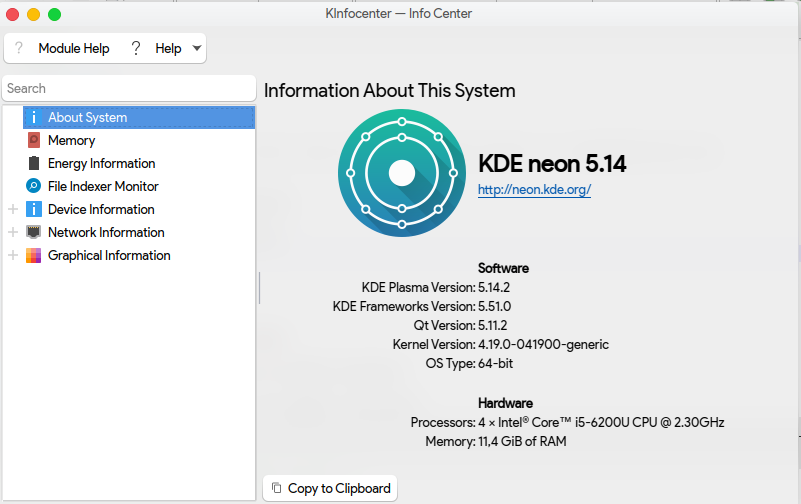
\includegraphics[scale=0.75]{imgs/machineA.png}
			\caption{Caractéristique de la machine de test}
			\label{fig:maxhineA}
		\end{figure}
		
		\subsection{Langage}
		\paragraph{}
	
		Pour la partie implémentation nous avons choisi le langage C++, car c'est un outil 
		de développement très performant et le plus puissant de sa génération, et qui jouit
		d'une grande rapidité d'exécution. C'est aussi un langage utilisant le paradigme 
		de la programmation orienté objet.
		
		\subsection{OpenCV}
		\paragraph{}
		\textbf{OpenCV }est une bibliothèque de traitement d'image en temps réel et de vision
		par ordinateur écrite en C/C++ , optimisée et proposée par \textbf{intel} pour Linux et
		Windows.
		\subsection{Qt framework}
		\paragraph{}
		\textbf{Qt} est une bibliothèque offrant le module GUI ( Graphical User Interface),
		conçue pour la création des interfaces graphiques. Elle offre aussi la possibilité
		de coder en C++ , JAVA , Python . . . etc.
	
	\section{Schéma global du système}
	Le système se compose principalement de trois modules:
	
	\begin{itemize}
		\item D’abord le module de détection récupère l’image de la caméra pour y détecter les couleurs recherchées et génère des informations sur le curseurs i.e sa position et son état.
		
		\item Le module de dessin reçoit les informations sur le curseur et les utilise pour générer l’image du dessin.
		
		\item Les deux modules précédents envoient leurs résultats à l’interface graphique pour l’affichage.
	\end{itemize}
	
	\begin{figure}[H]
		\centering
		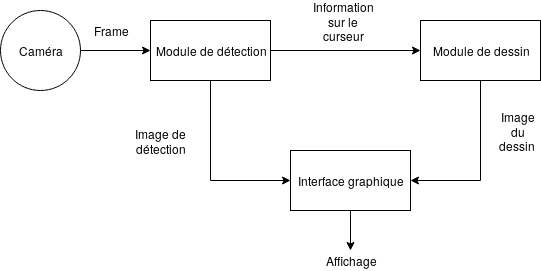
\includegraphics[scale=0.75]{imgs/MainDiagram.png}
		\caption{Schéma du système}
		\label{fig:SchemaGlob}
	\end{figure}
	
	\section{Détection de couleurs}
	\paragraph{}La détection de couleurs se fait sur une image en HSV, ceci est dû au fait que HSV sépare la valeur de teinte de celle de la luminosité ce qui le rend plus robuste envers les changements de lumière. 
	
	Ainsi la détection d’une des deux couleur se fait en passant par tous les pixels de l’image et décider pour chaque pixel s’il a la couleur recherché ou non. La décision se fait en testant l’appartenance du pixel à un intervalle de détection. Pour chacune des valeur H,S,V du pixel, on vérifie si cette valeur appartient à un intervalle définit lors du choix de l’utilisateur de la couleur à détecter comme suit: 
	
	Soit la couleur choisie H1S1V1, et le pixel candidat HSV, les conditions que doit vérifier le pixel sont:
	\begin{itemize}
		\item $H1-t \leq H \leq H1+t$ : l’intervalle de teinte dépend fortement de la couleur sélectionnée.
		
		\item $S1*0.6 \leq H \leq 255$: l’intervalle de saturation dépend légèrement de la couleur sélectionnée.
		
		\item $20 \leq H \leq 255$: On accepte un intervalle de luminosité large.
	\end{itemize}
	\paragraph{}Après avoir sélectionner les pixels qui ont la couleur désirée, on calcule le centre de ces pixels. Ainsi la détection résultera en deux centres, un pour chaque couleur. La distance entre ces deux derniers détermine si le curseur est active. Si la distance est supérieur à un seuil donné le curseur est désactivé, il est active sinon. Quant à la position du curseur elle est représenté par le centre des deux points sus-cités.\\
	\begin{figure}[H]
		\centering
		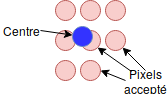
\includegraphics[scale=0.75]{imgs/centerExample.png}
		\caption{Exemple centre de détection}
		\label{fig:CenterCorrect}
	\end{figure}
	\textbf{Le problème} qui se pose en se limitant à la détection par intervalle c’est qu’elle est extrêmement sensible au bruit. Un pixel aberrant appartenant à l’intervalle va fausser la position du centre, et ainsi un suivi médiocre de la couleur.
	\begin{figure}[H]
		\centering
		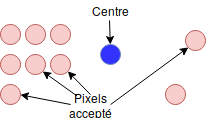
\includegraphics[scale=0.75]{imgs/centerExampleE.png}
		\caption{Exemple centre de détection avec bruit}
		\label{fig:CenterWrong}
	\end{figure}
	\section{Élimination du bruit par regroupement}
	\paragraph{}Pour remédier au problème rencontré, Nous avons opté à éliminer le bruit en regroupant les pixels proches qui sont acceptés. Avec cette méthode le bruit sera représenté par de petits groupes de pixels qu'on éliminera.\\
	L’algorithme de regroupement fonctionne comme suit:
	\begin{itemize}
		\item Il prend en paramètre un seuil minimum pour jugé que deux pixels appartiennent au même groupe.
		
		\item Au début chaque pixel est dans un groupe à part.
		
		\item L’algorithme passe par plusieurs itérations de regroupement, dans une itération chaque groupe de pixel est fusionné avec un autre dont la distance est inférieur au seuil modifié* s'il existe, ainsi on regroupe les pixels proches entre eux dans un seul groupe.
		
		\item L’algorithme s’arrête quand les groupes ne changent pas après une itération, ceci implique que tous les groupes sont éloignés entre eux.
	\end{itemize}
	\begin{figure}[H]
		\centering
		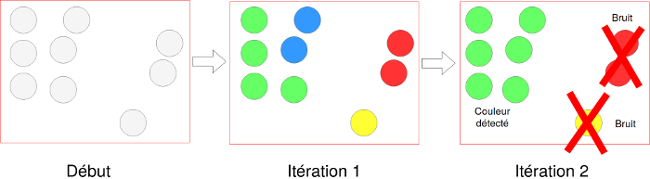
\includegraphics[scale=0.75]{imgs/grouping1.png}
		\caption{Exemple déroulement de l'algorithme de regroupement}
		\label{fig:Grouping}
	\end{figure}
	\paragraph{seuil modifié*:}Comme le seuil donné en entré est défini pour regrouper deux pixels, il est donc inadapté pour le fusionnement de deux groupes contenant plus d’un pixel. Le seuil doit être donc ajusté en fonction de la taille des groupes. Nous avons choisi d’utiliser la formule suivante: \textbf{$nouveauSeuil = (seuil/2)*(racine(tailleG1)+racine(tailleG2)$} avec \textbf{$tailleG1$} et \textbf{$tailleG2$} le nombre de pixels contenus par les groupes un et deux respectivement.\\
	L’intuition derrière cette formule, c’est que la distance entre deux centres de carrés collés est égale à $1/2*cote1+1/2*cote2$, avec cote1 et cote2 les cotés des deux carrés.
	\begin{figure}[H]
		\centering
		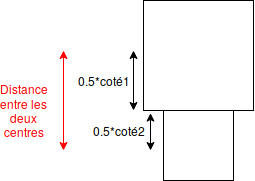
\includegraphics[scale=0.75]{imgs/distanceSquares.png}
		\caption{Exemple distance entre deux carrés collés}
		\label{fig:DistanceSquares}
	\end{figure}
	Dans notre cas, la taille du coté d’un pixel est l’unité de mesure de distance. La distance entre deux pixels peut être écrite en fonction de la taille de son coté comme suit: \textbf{$(distance/2)*(cotep+cotep)$} avec \textbf{$cotep$} la valeur d’un coté de pixel. Comme cotep=1 (l’unité de mesure) la formule précédente se réduit en la valeur de distance.
	\begin{figure}[H]
		\centering
		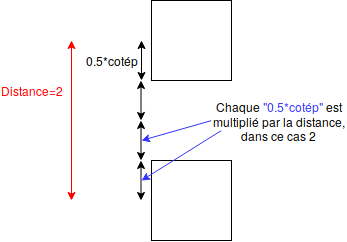
\includegraphics[scale=0.75]{imgs/distancePixels.png}
		\caption{Distance entre deux pixels représentant l'unité de mesure}
		\label{fig:DistancePixels}
	\end{figure}
	Si on projette cela sur un groupe de pixels carré, la taille de son coté est égale à la racine du nombre de pixels, car le nombre de pixels représente la surface du carré, ainsi la formule devient: \textbf{$(distance/2)*(racine(tailleG1)+racine(tailleG2)$}.
	\begin{figure}[H]
		\centering
		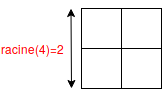
\includegraphics[scale=0.75]{imgs/GroupeSide.png}
		\caption{Exemple de coté d'un groupe de pixels}
		\label{fig:GroupeSide}
	\end{figure}
	\paragraph{Complexité}La complexité de l’algorithme est de $O(n²*log(n))$, $n$ étant le nombre de pixels acceptés. À chaque itération de l’algorithme pour chaque groupe on cherche un groupe avec lequel on le fusionne, au pire cas on passe par tous les groupes, et donc une complexité quadratique par itération. On fait $log(n)$ itération au max, car un groupe qui n’est pas fusionné lors d’une itération sera enlevé dans les prochaines itérations, donc au pire cas le nombre de groupes qui résulte d’une itération est égale au nombre de groupe initial divisé sur deux, cas où on fusionne les groupes deux par deux, d’où la complexité logarithmique.\\
	Il est à noter que l'opération de fusion se fait en $log(n)$ en utilisant une structure d'ensembles disjoints\footnote{plus d'information sur la structure d'ensembles disjoints: \href{https://en.wikipedia.org/wiki/Disjoint-set_data_structure}{https://en.wikipedia.org/wiki/Disjoint-set\_data\_structure}}.
	
	\paragraph{Inconvénients}
	
	Le premier inconvénient est le temps de calcule de l’algorithme. Si le nombre de pixels détecté par la première partie est important, la complexité quadratique ne convient pas à une détection en temps réel.\\
	
	Le deuxième inconvénient est le fait qu’on a besoin d’un seuillage pour faire le regroupement. Un seuil petit donne de bon résultat avec un grand intervalle de détection, il est robuste par rapport au bruit proche à l’objet qu’on suit. Par contre si l’intervalle de détection est petit, l’objet peut être divisé en deux groupes. Le contraire s’applique si le seuil est grand, un grand intervalle pourrait regrouper des pixels qui n’appartiennent pas à l’objet dans le même groupe que ce dernier.
	\section{Élimination du bruit par érosion et dilatation}
	Le principe de cette méthode est simple, on représente les pixels acceptés dans une image en niveau de gris, le pixel est blanc s’il est accepté et noir sinon. On applique une série d’érosions jusqu’à ce qu’on a que des pixels noir, et on garde la dernière image non nul. Dans cette dernière, les pixels non noir appartiennent probablement à l’objet qu’on veut détecter, avec l’hypothèse que l’arrière plan ne contient pas la couleur recherchée. La suite sera d’appliquer une série de dilatation tout en gardant en blanc que les pixels qui étaient blancs dans l’image d’origine, on s’arrête quand l’image ne change pas. Ainsi on est sur que les pixels en blanc après ces deux séries ont été détectés au préalable et qu’ils ont une forte chance d’appartenir à l’objet suivi.
	\begin{figure}[H]
		\centering
		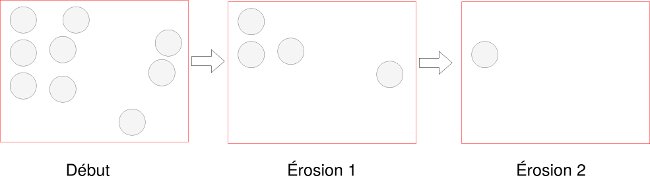
\includegraphics[scale=0.75]{imgs/erosions1.png}
		\caption{Exemple application d'une série d'érosions}
		\label{fig:Erosions}
	\end{figure}
	
	\begin{figure}[H]
		\centering
		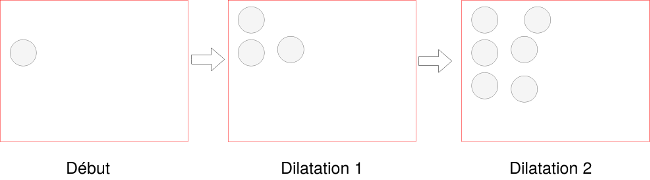
\includegraphics[scale=0.75]{imgs/dilatations1.png}
		\caption{Exemple application d'une série de dilatations}
		\label{fig:Dilatations}
	\end{figure}
	
	\chapter{Présentation de l'application}
	Dans ce chapitre nous allons détailler l’application qui utilise les méthodes présentées précédemment afin de permettre à un utilisateur de dessiner avec ses doigts.
	\section{Utilisation}
	\paragraph{}
	L’application commence d’abord par donner la main à l’utilisateur pour choisir les couleurs à détecter. Ceci se fait en les mettant dans une zone définie par l’application afin qu’elle puisse récupérer les couleurs à suivre.\\
	\begin{figure}[H]
		\centering
		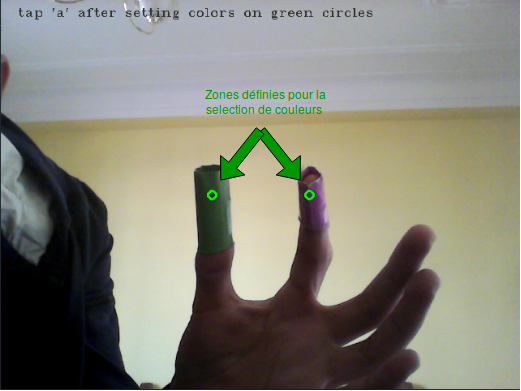
\includegraphics[scale=0.6]{imgs/initColors.png}
		\caption{L'étape initiation de couleurs à suivre}
		\label{fig:InitColors}
	\end{figure}
	\newpage
	L’interface contient principalement 3 parties:
	\begin{itemize}
		\item 1-2 :Options de l’application:
		\begin{itemize}
			\item Changer la méthode de détection, i.e par regroupement ou par série d’érosions/dilatations.
			\item Affichage des images de détections en niveau de gris.
		\end{itemize}
		\item 3 : Espace de dessin.
		\item 4 : Image récupéré par la caméra avec les centres des couleurs détectées.
	\end{itemize}
		\begin{figure}[H]
		\centering
		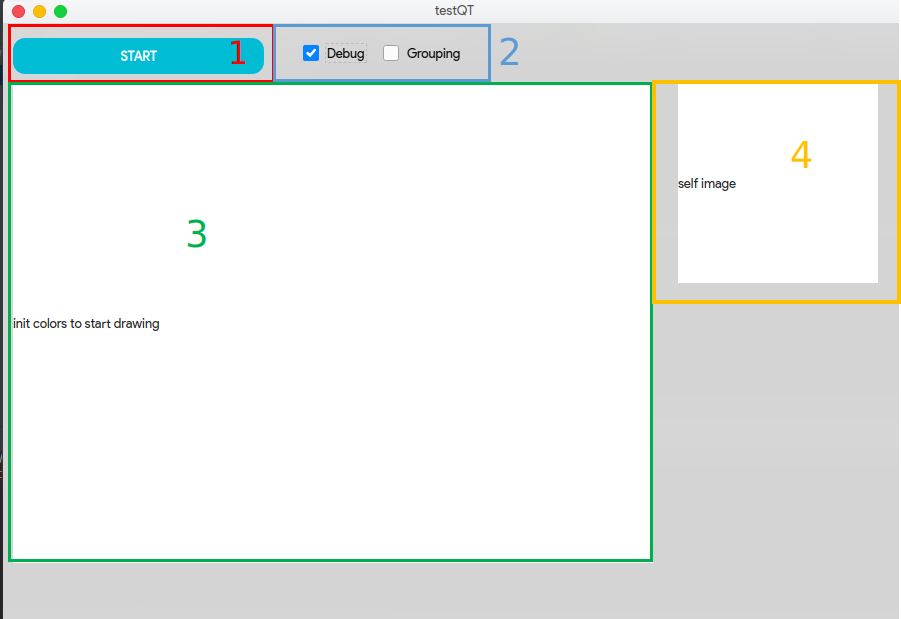
\includegraphics[scale=0.6]{imgs/main.png}
		\caption{Les partie de l'application}
		\label{fig:AppParts}
	\end{figure}

	\paragraph{Espace de dessin}
	Cette espace est géré principalement par le module de dessin cité dans le chapitre précédent. Ce module utilise juste l’information sur le curseur, sa position et son état d’activation, pour déterminer l’action à prendre. L’espace de dessin est composé de deux parties:
	\begin{itemize}
		\item La partie paramétrage dans laquelle on peut changer les paramètres du dessin.
		\item La partie feuille de dessin, c’est dans cette partie que l’utilisateur va réaliser son dessin.
		\begin{figure}[H]
			\centering
			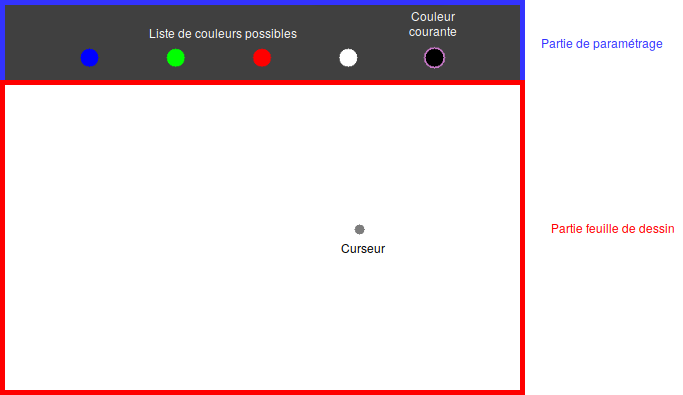
\includegraphics[scale=0.75]{imgs/Drawer.png}
			\caption{L'espace de dessin}
			\label{fig:Drawer}
		\end{figure}
	\end{itemize}
	
	Il existe 3 types d’actions que le module de dessin peut prendre:
	\begin{itemize}
		\item Dessiner: quand le curseur est active dans la partie feuille de dessin.
		\item Changer la couleur du curseur: s’il détecte un clique sur une couleur de la partie paramétrage qui est différente de la couleur courante.
		\item Changer la taille du curseur: s’il détecte un clique sur la couleur courante.  
	\end{itemize}
	\paragraph{}
	La dernière partie de l’interface graphique permet de visualiser comment les algorithmes de détection marche, par exemple on peut voir les groupes générés ainsi que leurs centres:
	\begin{figure}[H]
		\centering
		\begin{subfigure}{.5\textwidth}
			\centering
			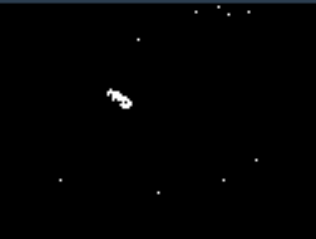
\includegraphics[width=.4\linewidth]{imgs/notGrouped.png}
			\caption{Les pixels acceptés sans regroupement}
			\label{fig:sub1}
		\end{subfigure}%
		\begin{subfigure}{.5\textwidth}
			\centering
			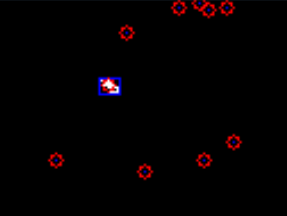
\includegraphics[width=.4\linewidth]{imgs/grouped.png}
			\caption{Les pixels acceptés avec regroupement}
			\label{fig:sub2}
		\end{subfigure}
		\label{fig:test}
	\end{figure}
	\section{Limitations}
	\paragraph{}
	Notre implémentation reste très limitée, elle souffre d'une sensibilité à la lumière
	ambiante, elle ne permet pas la présence d'un fond de la même couleur que les couleurs
	détectées dès la premières étape. l'absence de parallélisme est un grand défaut à lui
	tout seul.
\chapter{Conclusion générale}
\paragraph{}
À la fin de ce projet, nous avons pu nous initier à la vision par ordinateur, en utilisons à la fois
des techniques existantes, mais aussi une méthode que nous avons développé afin d'atteindre les
objectifs fixés au début du chapitre 1. Néanmoins malgré les efforts fournis, la porté de notre système
reste limitée, encore sujette à des conditions très strictes, nous espérons toute fois que ce travail
nous inspirera dans nos projets futurs en ne gardant que les points positifs et en apprenant de nos erreurs.



\end{document}}

